%% Data & Knowledge Engineering / Elsevier CAS manuscript package.
%% SC-FMA: Structurally-Calibrated Functional Attribution for Knowledge Engineering and Audit Prioritization
\documentclass[a4paper,fleqn]{cas-sc}

\usepackage[numbers,sort&compress]{natbib}
\usepackage{amsmath}
\usepackage{booktabs}
\usepackage{array}
\usepackage{graphicx}
\usepackage{xurl}
\usepackage{amsthm}
\newtheorem{theorem}{Theorem}[section]
\newtheorem{lemma}[theorem]{Lemma}
\newtheorem{corollary}[theorem]{Corollary}
\usepackage{algorithm}
\usepackage{algpseudocode}
\usepackage{multirow}
\usepackage{makecell}
\usepackage{placeins}
\usepackage{CJKutf8}
\usepackage{xr}
\usepackage{hyperref}
\hypersetup{colorlinks=true,linkcolor=blue,citecolor=blue,urlcolor=blue}
\externaldocument[][nocite]{supplementary}
\newcolumntype{Z}[1]{>{\raggedright\arraybackslash}p{#1}}
\newcommand{\wstruct}{\ensuremath{\mathbf{w}_{\mathrm{struct}}}}

\begin{document}
\let\WriteBookmarks\relax
\def\floatpagepagefraction{1}
\def\textpagefraction{.001}
\pagenumbering{arabic}

\shorttitle{Structurally-Calibrated Functional Attribution}
\shortauthors{Ma and Wang}

\title[mode=title]{Structurally-Calibrated Functional Attribution for Audit Prioritization in Knowledge-Intensive Reasoning}

\author[1]{Haoran Ma}
\ead{mahaoran0000@foxmail.com}

\author[1,2]{Ningning Wang\corref{cor1}}
\ead{wangningning@bistu.edu.cn}

\cortext[cor1]{Corresponding author.}
\renewcommand{\printorcid}{}

\affiliation[1]{organization={College of Management Science and Engineering, Beijing Information Science and Technology University},
            city={Beijing},
            postcode={102200},
            country={China}}

\affiliation[2]{organization={Institute of Information Systems, ESG Intelligent Application Innovation Research Center},
            city={Beijing},
            postcode={102200},
            country={China}}

\begin{abstract}
Knowledge-intensive systems increasingly expose intermediate knowledge artifacts, including reasoning traces, graph nodes, process annotations, retrieval checks, entity bindings, and verification records. These artifacts must be represented and maintained under limited curation budgets, but they are often available only as heterogeneous signals rather than reusable audit records. Existing PRM and process-supervision methods provide step-level annotation signals, scalar attribution methods estimate local influence, and graph-based salience methods identify structurally exposed nodes. What they do not provide is a knowledge representation layer that transforms heterogeneous intermediate artifacts into decomposed, queryable audit records under a fixed budget. We introduce Structurally-Calibrated Functional Attribution (SC-FMA), a knowledge artifact transformation framework for fixed-budget knowledge audit prioritization. SC-FMA represents artifacts as dependency-aware audit graphs and uses the Structurally-Calibrated Utility (SCU) objective to construct records that preserve annotation or utility fidelity while exposing structural dependency, redundancy, bottleneck, audit-reason, and maintenance-action fields. The validation instantiates a knowledge engineering task formulation for fixed-budget audit of intermediate knowledge artifacts, covering structured audit-priority allocation, representation sensitivity to graph construction, and audit-record construction. On a locked PRM800K annotation distribution with 4,417 samples and 34,219 labeled steps, SC-FMA Ridge closely preserves the strongest supplied fidelity field (Spearman $\rho=0.604$ versus $0.611$ for \wstruct{}) while exposing decomposed audit fields; QP and Projection are lower-consistency variants on this real-data distribution. A Countries-KG study shows that ontology-derived edges can change structural-dependency allocation, and a rule-derived audit-target retrieval stage improves budget-constrained coverage from 0.235 to 0.699 over a scalar-only view, with circularity explicitly bounded by target type. SC-FMA therefore provides a knowledge engineering layer for converting intermediate knowledge artifacts into structured audit records for fixed-budget knowledge maintenance and curation.
\end{abstract}

\begin{keywords}
knowledge engineering \sep knowledge representation \sep knowledge maintenance \sep knowledge graphs \sep audit prioritization \sep functional attribution
\end{keywords}

\maketitle

\section{Introduction}

Knowledge-intensive systems increasingly expose intermediate artifacts during reasoning, retrieval, annotation, validation, and update. These artifacts include reasoning traces, graph nodes, entity bindings, verification records, rule-like operations, retrieval checks, and process annotations. They are not merely transient model outputs: once exposed, they become knowledge artifacts that must be represented, organized, maintained, curated, and reused. The practical challenge is that these artifacts often exceed the audit capacity available to curators, while maintenance decisions must still be made under fixed review budgets.

Existing methods address only parts of this knowledge engineering problem. PRM and process-supervision methods attach scalar quality signals to reasoning steps, but they do not convert those steps into structured maintenance records. Local utility-signal methods estimate artifact influence, but they do not distinguish whether an artifact should be inspected because it provides local evidence, supports a dependency, duplicates existing support, or exposes a downstream bottleneck. Graph-based salience methods can identify structurally prominent nodes, but they do not integrate process annotations, utility signals, and curation actions into a reusable audit representation. Consequently, these methods can produce priorities, but they cannot specify what the artifact is, why it matters in the knowledge structure, and what maintenance action a fixed-budget audit should take.

This paper introduces Structurally-Calibrated Functional Attribution (SC-FMA) as a knowledge representation transformation layer for this setting. SC-FMA transforms observable intermediate knowledge artifacts into structured audit records by representing their dependencies, calibrating supplied annotation or utility signals, and attaching explicit audit reasons and maintenance actions. Audit-priority allocation is therefore a downstream use of the representation, not the identity of the method. The central contribution is to make audit prioritization a representation problem: SC-FMA enables fixed-budget knowledge maintenance over structured artifacts by converting raw traces, graph relations, and process annotations into dependency-aware records that can be inspected, queried, curated, and reused.

The paper makes three contributions. First, it formulates fixed-budget audit prioritization for structured knowledge artifacts, where intermediate records must be selected for review under limited curation resources. Second, it introduces SC-FMA and the SCU objective, which combine annotation fidelity, structural dependency, redundancy, and bottleneck roles into decomposed audit records. Third, it evaluates the representation on PRM800K annotation evidence, a Countries-KG knowledge-graph representation study, rule-derived audit-target retrieval, and controlled synthetic calibration, keeping deployment and downstream-training claims separate from the reported audit-prioritization evidence.

The main findings follow the same knowledge-engineering workflow. On PRM800K annotation evidence (4,417 samples and 34,219 labeled steps under a frozen hash split), \wstruct{} is treated as a fidelity field for artifact prioritization, and SC-FMA Ridge closely preserves annotation-order consistency (Spearman $\rho = 0.604$ versus $0.611$) while exposing decomposition fields for audit; this is a preservation-with-decomposition result, not a predictive-improvement result over \wstruct{}. The Countries-KG study shows that typed ontology edges can change structural-dependency allocation at the graph-representation interface. Rule-derived audit-target retrieval shows that SC-FMA decomposition exposes bottleneck, redundancy, weak-anchor, and structural-overcorrection targets more fully than a scalar-only view under the same fixed audit budget, but these targets are automatic rules rather than human adjudications and three target families share partial circularity with the decomposition fields. Controlled synthetic calibration and ablation explain when structural fields affect audit-priority allocation and when they mainly provide regularization and audit-record decomposition.

The remainder of this paper is organized as follows. Section~\ref{sec:related-work} reviews attribution, step-level annotation signals, graph-based knowledge engineering, and audit methods. Section~\ref{sec:methods} presents SC-FMA, the SCU objective, and its theoretical properties. Section~\ref{sec:experimental-results} reports knowledge-engineering task validation from real annotation evidence to knowledge-graph representation and controlled calibration. Section~\ref{sec:discussion} interprets the method in the knowledge lifecycle, and Section~\ref{sec:conclusions} concludes.

Figure~\ref{fig:overall-framework} gives the high-level knowledge-engineering workflow. SC-FMA sits between raw knowledge artifacts and downstream maintenance actions: it represents artifacts as dependency graphs, calibrates annotation signals with SCU, and returns knowledge audit records with explicit structural roles and maintenance actions.

\begin{figure}[pos=ht]
\centering

\includegraphics[width=\linewidth]{figures/fig_overall_framework.pdf}
\caption{Knowledge engineering workflow for SC-FMA. The figure should be read as a transformation from Knowledge Artifact $\rightarrow$ Representation $\rightarrow$ Graph Structure $\rightarrow$ SCU $\rightarrow$ Audit Record $\rightarrow$ Knowledge Curation. Raw reasoning traces, graph nodes, and process annotations are first organized as auditable knowledge artifacts, then represented through dependency-aware graph structure. SCU constructs structured audit records by preserving annotation or utility fidelity while adding structural dependency, redundancy, bottleneck, audit-reason, and maintenance-action fields. The resulting records support fixed-budget knowledge maintenance and curation; audit-priority allocation is only a downstream use of the audit representation.}
\label{fig:overall-framework}
\end{figure}

\section{Related Work}
\label{sec:related-work}

\subsection{Attribution and Explanation}

Attribution methods ask which parts of an input, computation, or structure matter for a decision. Integrated Gradients attributes predictions to input features along a path from a baseline~\cite{sundararajan2017axiomatic}; SHAP unifies additive feature-attribution methods~\cite{lundberg2017unified}; and LIME explains individual predictions through local interpretable surrogates~\cite{ribeiro2016lime}. Rationale-oriented work such as ERASER evaluates extractive spans rather than only continuous attribution values~\cite{deyoung2020eraser}.

Structure-aware attribution adds another layer. Network studies show that importance can be non-local, redundant, or concentrated around bottleneck nodes~\cite{albert2000error,newman2010networks}. For graph models, GNNExplainer selects compact subgraphs that explain predictions~\cite{ying2019gnnexplainer}. User-centered explanation work further shows that an explanation is useful only when it matches the reviewer's task~\cite{kaplan2024xai}.

These lines motivate SC-FMA but leave a gap for audit triage. Salience identifies important evidence, yet it does not specify whether the reviewer should inspect local support, consolidate duplicated evidence, protect a downstream dependency, or repair a weak upstream signal. Entailment-tree methods move explanation toward intermediate justifications~\cite{dalvi2021entailmenttrees}, and counterfactual methods move it toward contrastive evidence~\cite{wijekoon2023counterfactual}. SC-FMA keeps these audit roles separate.

\subsection{Process Supervision and Process Reward Models}

Process supervision assigns annotation signals to intermediate steps rather than only final answers. PRM800K showed that process reward models trained on per-step human labels can provide stronger verifier-guided best-of-$N$ search behavior than outcome reward models~\cite{lightman2023verify}. The GSM8K verifier setup made this training route concrete~\cite{cobbe2021training}, and process-based feedback reduced reasoning errors even when outcome success appeared saturated~\cite{uesato2022solving}. These studies provide the kind of step-resolved fidelity signal that SC-FMA can calibrate.

A parallel line makes verification, critique, and revision themselves available as annotated process units. Chain-of-thought prompting elicits intermediate reasoning~\cite{wei2022cot}, and self-consistency aggregates multiple sampled chains into a more reliable signal~\cite{wang2022selfconsistency}. Tree of Thoughts extends search from linear chains to deliberate tree-structured exploration~\cite{yao2023tot}, while ReAct interleaves reasoning and acting for verification~\cite{yao2022react}. On the revision side, Reflexion~\cite{shinn2023reflexion} and Self-Refine~\cite{madaan2023selfrefine} introduced reflective agents that critique and revise their own outputs, turning revision steps into an additional supervision target.

Recent process-diagnostic resources also show that step-level signals need distributional checks. Math-Shepherd studies automatic step verification without human annotations~\cite{wang2024mathshepherd}, and ProcessBench evaluates process-error identification across models~\cite{zheng2024processbench}. These resources help assess scalar step signals. SC-FMA treats such signals as inputs to structural calibration rather than as final explanations.

\subsection{Graph-Based Knowledge Engineering and Audit Methods}

Graph-based knowledge engineering shows how structured intermediate states can be made inspectable. Knowledge-engineering methods have long treated representation, inference, and maintenance as coupled design problems~\cite{studer1998knowledge}. Classic rule-based systems treated auditability as a design principle: MYCIN exposed certainty-factor chains that connected conclusions to rules~\cite{buchanan1984mycin}, and DENDRAL exposed generate-and-test plans for chemical structure enumeration~\cite{lindsay1980dendral}. Cognitive architectures such as Soar and ACT-R also made internal states and operator applications available for step-level review~\cite{laird2012soar,anderson2004actr}.

Modern knowledge-intensive pipelines shift the review focus from hand-built rules to learned workflows that connect language models with structured knowledge. Knowledge graphs provide a general representation substrate for entities, relations, constraints, and graph-level quality signals~\cite{hogan2021knowledge}. RAG exposes retrieved passages as evidence~\cite{lewis2020rag}, and survey work documents the broader family of RAG variants~\cite{gao2023ragsurvey}. GraphRAG builds entity graphs and pre-generates community summaries for global queries~\cite{edge2024graphrag}. KG-RAG connects a pre-existing knowledge graph to LLM generation through chain-of-exploration reasoning~\cite{sanmartin2024kgrag}. Knowledge-enhanced language models and LLM-KG integration further expose entity links, triples, relation paths, and graph-quality signals as knowledge artifacts for audit~\cite{hu2024knowledgeenhanced,pan2024unifying,yang2025kbllmsurvey,chen2025kgquality,dai2025llmkg}. Similar audit pressure appears in long-tail KG-augmented question answering and engineering-design RAG, where sparse factual support and heterogeneous evidence make exhaustive review unrealistic~\cite{huang2025prompting,siddharth2024retrieval,liu2025knowledgereasoning}.

Across these settings, the challenge is no longer simply recovering intermediate evidence. Modern pipelines already expose passages, entity links, relation paths, and verification records. The harder question is how a reviewer should allocate a limited curation budget across them and how the resulting records should support refinement, update, and reuse~\cite{paulheim2017knowledge,higgins2008dcc}. SC-FMA connects to this knowledge-engineering audit tradition by converting exposed artifacts into graph-aware audit records.

\subsection{Summary of Research Gap}

Existing work supplies three ingredients: local attribution identifies salient evidence, process supervision supplies step-level annotation fidelity, and graph-based knowledge engineering exposes structural context. SC-FMA combines them into a representation layer that turns exposed knowledge artifacts into inspectable records for fixed-budget knowledge audit.

\section{Method}
\label{sec:methods}

\subsection{Workflow Overview}

\textbf{Representation Transformation Statement.} SC-FMA transforms raw intermediate reasoning artifacts into structured, queryable knowledge audit representations. The method should be read as a knowledge representation layer between exposed artifact streams and downstream maintenance actions, not as a standalone prioritization heuristic. SCU does not define a scalar decision rule, but defines a structured representation constraint system over knowledge artifacts.

The input is a set of observable knowledge artifacts such as retrieval checks, entity bindings, rule-like operations, verification records, or reflective annotations. These artifacts are first normalized into an auditable artifact sequence, converted into a graph representation with temporal and optional domain edges, calibrated by SCU against the supplied annotation or utility signal, and emitted as knowledge audit records. A downstream curator can then use those records to allocate a fixed audit budget while seeing both the audit-priority value and the maintenance reason for inspection.

\subsection{SC-FMA as a Representation Layer}

Unlike conventional scalar attribution methods, SC-FMA explicitly represents structural dependencies among intermediate knowledge artifacts and converts them into audit-oriented knowledge records. The method acts as a representation layer between raw artifacts and downstream maintenance actions: it does not replace the reasoning system, the retriever, the knowledge graph, or the annotator, but reorganizes their exposed outputs into records that preserve fidelity information while adding structural role and maintenance-action fields.

\subsection{Formal Problem Definition}

\textbf{Input.} SC-FMA takes an observable artifact sequence $T=(s_1,\ldots,s_k)$, where each unit $s_i$ may be a verification, reflection, retrieval, entity-binding, or rule-like operation available for audit. The sequence is converted into a graph $G=(V,E)$ whose nodes correspond to artifact units and whose edges encode temporal adjacency plus optional topical or domain-specific relations. The method also receives a utility or fidelity signal $u$ over the same units. This signal may come from local utility estimation, a proxy representation signal, or a learned step-annotation model, and SC-FMA treats it as the fidelity signal to be preserved when it is informative.

\textbf{Output and objective.} The output is a set of calibrated knowledge artifact records. Each record contains an audit-priority field plus fidelity, structural-dependency, redundancy, bottleneck, audit-reason, and maintenance-action fields. The methodological object is the structured record rather than a priority list alone. The objective is to preserve useful utility signal, incorporate observable artifact structure, and attach each selected artifact to a concrete audit action.

\subsection{SCU Objective and Audit Decomposition}
\label{sec:scu-objective}

The SCU objective is designed to produce an executable audit representation, not merely a scalar priority value. Its role is to preserve an informative fidelity signal while making the structural reason for each priority visible under a fixed budget. Dependency, redundancy, and bottleneck fields therefore do not serve as decorative metadata; they determine whether a selected knowledge artifact should be checked as local evidence, protected as a dependency, consolidated as repeated support, or retained because later artifacts depend on it.

For an artifact sequence with $k$ auditable units, let $\tilde{\mathbf{c}}\in\mathbb{R}^k$ denote the normalized utility or proxy-fidelity input. In the PRM800K locked stage, \wstruct{} denotes the frozen Ridge regressor used as this fidelity signal. In the binary-correctness diagnostic setting, $\tilde{\mathbf{c}}$ is a coarse sequence-level local utility anchor: it records how an observed outcome changes under a documented intervention. Let $\tilde{\mathbf{n}}$ denote normalized structural necessity from graph perturbation diagnostics, $\mathbf{R}$ a redundancy matrix, and $\mathbf{b}$ a bottleneck indicator.

SC-FMA computes audit-allocation values $\mathbf{w}$ on the probability simplex
\begin{equation}
\mathcal{W}=\{\mathbf{w}\in\mathbb{R}_{+}^{k}: \sum_i w_i = 1\}
\label{eq:scu-feasible-set}
\end{equation}
by minimizing the SCU objective:
\begin{equation}
L(\mathbf{w}) =
\alpha\|\mathbf{w} - \tilde{\mathbf{c}}\|_2^2
+ \beta\|\mathbf{w} - \tilde{\mathbf{n}}\|_2^2
+ \gamma\,\mathbf{w}^{\top}\mathbf{R}\mathbf{w}
- \delta\sum_i b_i \log(w_i).
\label{eq:scu}
\end{equation}
Unless otherwise stated, $\alpha,\beta,\gamma,\delta \ge 0$ and $\mathbf{R}$ is treated as symmetric positive semidefinite on the feasible subspace. The four terms encode fidelity to the supplied input, structural alignment, redundancy regularization, and non-zero bottleneck regularization. The fidelity signal consistently provides the dominant optimization signal. The redundancy penalty and bottleneck log-barrier mainly act as regularization terms that encourage interpretable decomposition fields, although their quantitative contribution to audit-priority consistency is modest under the current validation setting. Detailed notation, construction rules, algorithms, and proofs are provided in the supplementary material.

\subsection{Artifact Representation}

Each artifact sequence is represented as an ordered set of auditable knowledge artifacts. The current implementation supports units derived from structured reflection tags and free-text chain-of-thought segmentation. In this paper, segmentation is treated as an observed input rather than a solved NLP problem.

A node $v_i$ corresponds to one artifact unit. Temporal edges connect adjacent units, while topical edges connect units whose TF-IDF similarity exceeds the configured threshold. The graph serves as a representation substrate for knowledge dependencies rather than a feature-extraction pipeline; TF-IDF is only the lightweight default backend for constructing lexical dependency cues when richer domain relations are unavailable. This temporal-plus-topical graph is the default SCU instantiation for text-only artifact sequences and gives the method an auditable structural record.

A supplementary graph-construction ablation replaces TF-IDF topical edges with Sentence-BERT embeddings (\texttt{sentence-transformers/all-MiniLM-L6-v2}, 384 dimensions). In that 800-trace fixture, the TF-IDF topical default (0.0515) did not exceed temporal-only edges (0.0596) on diagnostic structural-necessity consistency, while the embedding backend (0.0615) slightly improved the same diagnostic readout.

These differences are too small to treat topical edges as an audit-priority allocation driver. We therefore read the graph layer as an interchangeable \emph{construction interface}, not as evidence that the TF-IDF topology adds priority-allocation value over the temporal chain.

The graph constructor is modular. Richer domain-specific backends --- semantic embeddings, entity links, knowledge graphs, ontologies, rule-dependency DAGs, and data-lineage graphs --- can replace the default without modifying the SCU objective. The Countries-KG representation study (Section~\ref{sec:kg-pilot}) and the embedding ablation illustrate this interface. The resulting graph is a directed acyclic approximation of an observable artifact sequence and serves as a reproducible audit graph.

\subsection{Structural Necessity, Redundancy, and Bottlenecks}

Structural necessity measures how much graph support is lost when a node is perturbed under a documented graph-level operation. The implementation uses PRUNE, CASCADE, and BYPASS diagnostics. PRUNE removes direct node support. CASCADE propagates disruption to downstream neighbors. BYPASS asks whether alternative paths can substitute for the removed artifact unit. The final necessity input $\tilde{\mathbf{n}}$ is the normalized summary of these observable graph diagnostics.

The redundancy matrix $\mathbf{R}$ captures pairwise similarity between artifact units. High redundancy means that two units appear to serve overlapping functions in the observed sequence. The penalty $\mathbf{w}^{\top}\mathbf{R}\mathbf{w}$ discourages allocating large budget share to many mutually redundant units at once. In the current evidence package, this term is best interpreted as a regularization and decomposition term: it records a possible duplicated-audit allocation pressure, but its direct contribution to audit-priority consistency is modest.

Bottleneck detection addresses the opposite diagnostic pattern. Some nodes are not redundant, and their downstream exposure can make them useful to inspect even if the supplied fidelity signal is modest. The log-barrier term prevents identified bottleneck nodes from being assigned near-zero audit allocation. In knowledge-base maintenance terms, this keeps a single point of failure visible to the reviewer. The term enforces a conservative audit regularizer when observed structure marks the node as difficult to replace.

Figure~\ref{fig:local-utility-necessity} illustrates the local-utility--necessity mismatch. Figure~\ref{fig:variant-behavior} reports the three perturbation modes, and Figure~\ref{fig:resilience} shows the resilience curves.

\begin{figure}[pos=ht]
\centering
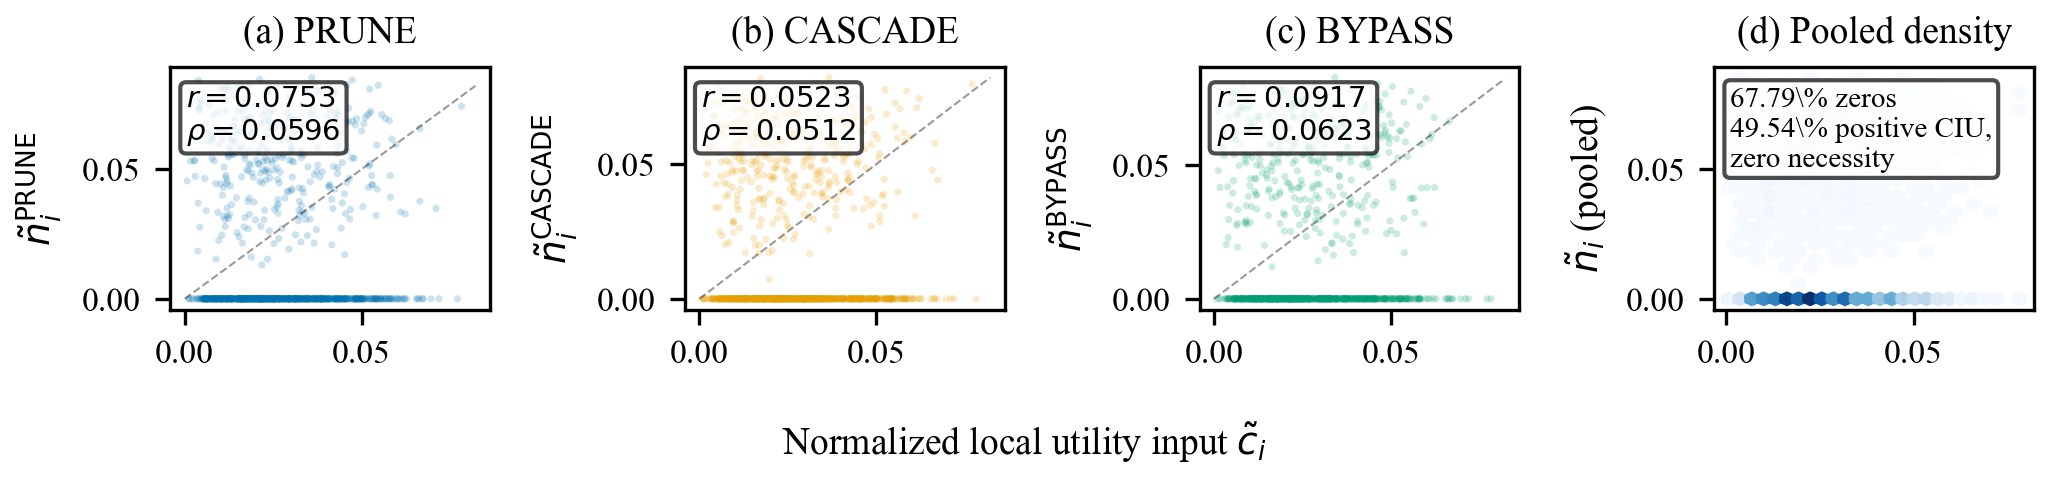
\includegraphics[width=\linewidth]{figures/fig_local_utility_necessity.png}
\caption{Structural diagnostic motivating calibration. Local utility and graph-level necessity are not interchangeable: many locally useful steps have low measured structural necessity, while some structurally exposed steps do not receive strong local utility signals. The shared $x$-axis $\tilde{c}_i$ denotes the normalized local utility input for step $i$. SC-FMA uses this mismatch as the reason for calibration.}
\label{fig:local-utility-necessity}
\end{figure}

\begin{figure}[pos=ht]
\centering
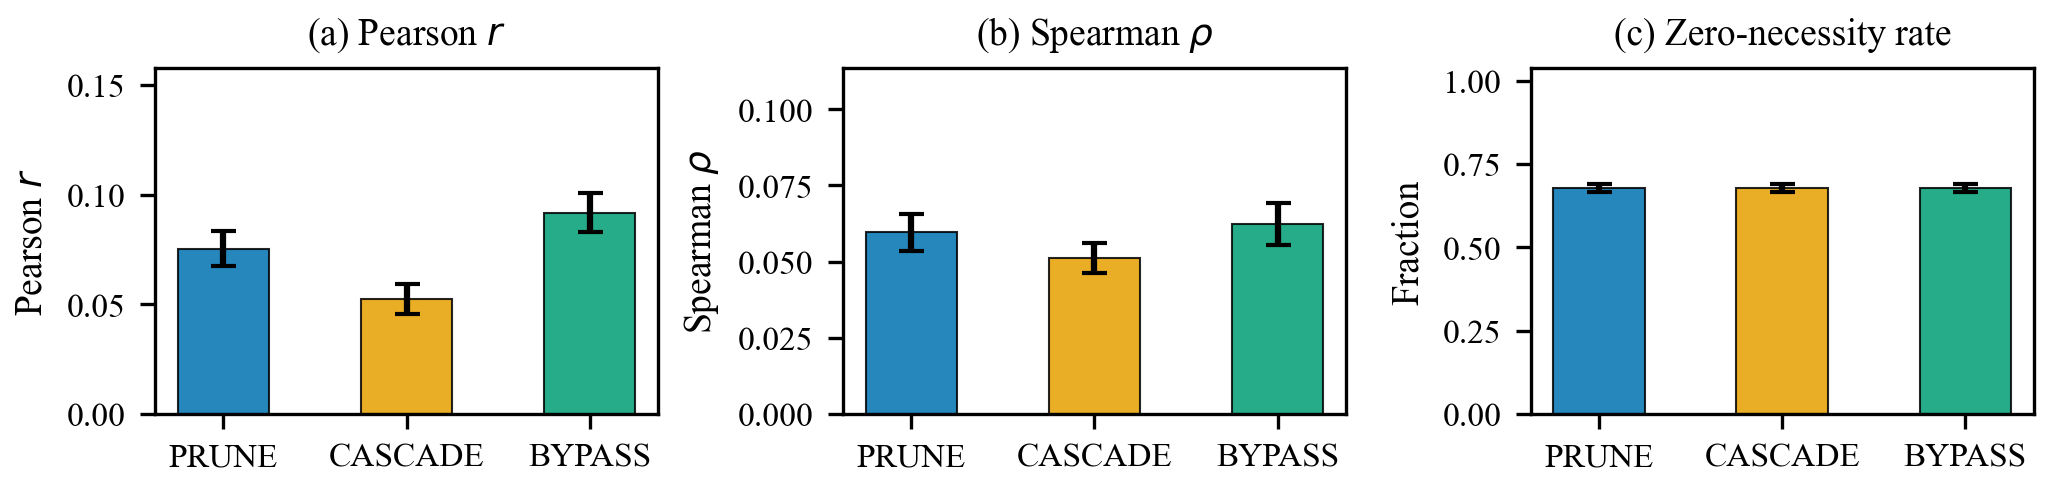
\includegraphics[width=\linewidth]{figures/fig_representation_variant_behavior.png}
\caption{Structural diagnostic summary by perturbation mode. The three perturbation modes (PRUNE, CASCADE, BYPASS) are reported with Pearson correlation, Spearman audit-priority consistency, and zero-necessity fraction. Error bars indicate 95\% bootstrap confidence intervals. The consistency across modes indicates that weak local-utility--necessity alignment is not an artifact of a single perturbation strategy.}
\label{fig:variant-behavior}
\end{figure}

\begin{theorem}[SCU well-posedness]
\label{thm:scu-well-posedness}
Assume $\alpha,\beta,\gamma,\delta \ge 0$ and $\mathbf{R}\succeq 0$ on the simplex tangent subspace. Then the SCU objective in Eq.~\ref{eq:scu} is convex on the relative interior of the simplex in Eq.~\ref{eq:scu-feasible-set}. If $\alpha+\beta>0$, or if $\gamma\mathbf{R}$ is positive definite on the tangent subspace when $\alpha+\beta=0$, the quadratic part is strictly convex on the feasible subspace and the minimizer is unique. If $\delta>0$ and $b_i=1$, any finite minimizer assigns $w_i>0$ to that bottleneck node; the barrier therefore gives an interior guarantee for active bottleneck support. For non-redundant artifact-unit pairs with identical redundancy profiles and inputs ordered in the same direction, $\tilde c_i\ge \tilde c_j$ and $\tilde n_i\ge \tilde n_j$, the two-input allocation relation is monotone before redundancy-induced redistribution. This monotonicity is a diagnostic property, not a global ordering guarantee once redundancy profiles differ.
\end{theorem}

We implement three variants of the same calibration procedure; they are not competing claims that one optimizer is universally best. SC-FMA Ridge uses a closed-form softmax over a linear combination of $\tilde{\mathbf{c}}$ and $\tilde{\mathbf{n}}$. SC-FMA QP solves the full constrained program with redundancy and bottleneck terms. SC-FMA Projection applies a fast topology-constrained simplex projection onto the probability simplex~\cite{wang2013projection}. The validation sections report where each variant is appropriate.

The calibrated allocation field is meant to be inspectable. For each selected artifact unit, the implementation can report whether the priority was driven mainly by fidelity, structural dependency, redundancy regularization, or bottleneck regularization.

This decomposition maps priorities to curation actions. A high-fidelity object may support a positive annotation signal; a high-dependency object may require manual review despite modest local utility; a redundant group may be audited as a cluster; and a bottleneck object may deserve conservative retention because later reasoning depends on it.

SC-FMA does not imply that the largest allocation value is the only important artifact in a sequence. The simplex constraint represents an audit budget, so increasing one unit's allocation value decreases another unit's share of attention. The output is therefore a fixed-budget audit record with explicit allocation fields. Redundant artifact units should not all receive high allocation values, while isolated downstream-exposed units should not disappear from review.

\begin{figure}[pos=ht]
\centering
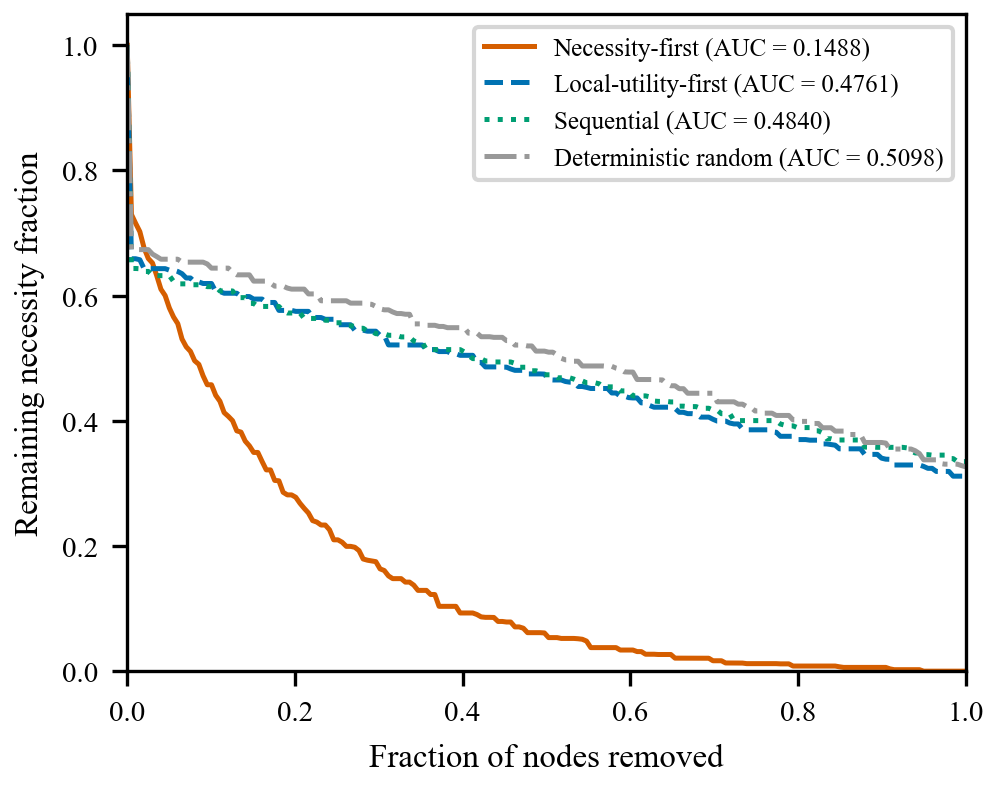
\includegraphics[width=0.88\linewidth]{figures/fig_resilience.png}
\caption{Resilience curves under ordered node removal. Four removal orders are reported: necessity-first, local-utility-first, sequential (original trace order), and deterministic random (hash-based). The $y$-axis shows remaining structural necessity fraction; the $x$-axis is the fraction of nodes removed. AUC values are annotated. The necessity-first curve degrades sharply (AUC $0.1488$), while local-utility-first (AUC $0.4761$) is close to random (AUC $0.5098$), showing that structural criticality requires graph-level diagnostics beyond local utility.}
\label{fig:resilience}
\end{figure}

\subsection{Role of Structural Components}

The structural components are not designed to exceed a strong fidelity signal in every setting. Their role is to preserve useful annotation signal when the fidelity field is strong and add audit information that a scalar-only view cannot expose: local support, structural exposure, redundancy, and bottleneck protection.

A fidelity-only scalar indicates which artifact receives attention but collapses the rationale. SC-FMA changes the interpretability of the audit record even when the allocation field changes only modestly: the contribution is preservation with decomposition.

\subsection{Computational Profile}

Empirical runtime is reported separately from the asymptotic summaries. In the frozen local artifacts, the PRM800K audit-prioritization run over 4,417 traces and 34,219 steps completed in 131.57\,s. Separately logged graph-construction, SCU component, and failure-taxonomy runs are reported in Appendix~\ref{app:runtime-reproducibility}.

\begin{table}[ht]
\caption{Asymptotic time complexity for SC-FMA fixed-budget audit. Here $N$ is the number of artifact sequences, $k$ is the number of auditable units in a sequence, $L$ is text length, $d$ is the sparse text-feature dimension, and $I$ is the number of QP solver iterations.}
\label{tab:complexity-summary}
\centering
\small
\renewcommand{\arraystretch}{1.08}
\begin{tabular}{p{0.36\linewidth}p{0.34\linewidth}p{0.20\linewidth}}
\toprule
\textbf{Stage} & \textbf{Input size} & \textbf{Time complexity} \\
\midrule
Artifact feature extraction & $N$ sequences, $k$ units, text length $L$ & $O(NkL)$ \\
Graph construction & $k$ nodes, sparse TF-IDF features $d$ & $O(k+k^2d)$ \\
Redundancy and bottleneck diagnostics & $k$ units, similarity matrix & $O(k^2d)$ \\
Ridge calibration & $k$ artifact-feature rows & $O(k)$ after learned coefficients \\
QP calibration & $k$ units, dense constraints & $O(Ik^3)$ worst case \\
Fixed-budget audit-priority allocation & $k$ audit-allocation fields & $O(k\log k)$ \\
\bottomrule
\end{tabular}
\end{table}

\begin{table}[ht]
\caption{Memory profile for the same pipeline stages. Dense graph quantities are shown for clarity; the implementation uses sparse storage where applicable.}
\label{tab:memory-summary}
\centering
\small
\renewcommand{\arraystretch}{1.08}
\begin{tabular}{p{0.46\linewidth}p{0.38\linewidth}}
\toprule
\textbf{Stage} & \textbf{Memory complexity} \\
\midrule
Artifact feature extraction & $O(k+d)$ per sequence \\
Graph construction & $O(k^2)$ dense; sparse in implementation \\
Redundancy and bottleneck diagnostics & $O(k^2)$ \\
Ridge calibration & $O(k)$ \\
QP calibration & $O(k^2)$ \\
Fixed-budget audit-priority allocation & $O(k)$ \\
\bottomrule
\end{tabular}
\end{table}

\FloatBarrier

\section{Knowledge Engineering Task Validation}
\label{sec:application}
\label{sec:experimental-results}

This section instantiates fixed-budget knowledge audit as a knowledge-engineering task. It evaluates representation behavior under fixed-budget knowledge-audit conditions, not model-comparison performance; correlation and retrieval metrics are used as fidelity and audit-coverage diagnostics for the resulting records. The validation suite examines three representation questions: whether audit records preserve useful annotation signals, whether graph construction changes structural-dependency representations, and whether decomposed records improve audit-target retrieval under budget constraints. Each stage follows the workflow in Figure~\ref{fig:overall-framework}: represent intermediate knowledge artifacts, construct an audit graph, calibrate an annotation or utility signal, and return an audit record. We begin by defining the fixed-budget audit task, then study PRM800K representation behavior, graph-based representation sensitivity, audit-record construction, controlled calibration, and failure modes of the representation layer.

\subsection{Task Definition: Fixed-Budget Knowledge Audit}
\label{sec:application-setup}

\subsubsection{Data Sources and Reference Views}

The PRM800K locked stage uses process-supervision annotations under the frozen v3.6/v3.8 hash split (4,417 samples and 34,219 labeled steps). Here process supervision is treated as a source of step-level annotation signals, not as the paper's main contribution. The hash split fixes sample assignment before locked validation to avoid post hoc selection. The Countries-KG stage uses a real knowledge graph as a representation-backend study. The controlled synthetic stage contains 200 traces generated with five fixed seeds (42, 123, 456, 789, 1024), with approximately 1,000 reflective steps per seed, and is used for representation calibration, ablation, and error analysis. Controlled annotation targets combine local correctness, lexical diversity, position, and graph-derived necessity. MuSiQue is reported as a supplementary constructed-label feasibility demonstration because its labels and feature fields share \texttt{step\_type}; full metrics and execution details are reported in the supplementary material. WebQSP trace-audit artifacts are reported as a supplementary fixed-schema diagnostic on executable traces (494 train traces for development and 1,627 locked test traces). GSM8K/HotpotQA task-specific replay and downstream filtering attempts are retained as failed or incomplete validation attempts.

Reference views include raw local utility, span length, relative position, seeded random allocation, and stage-specific scalar or feature-only views. Token-level attribution families such as gradient attribution, attention rollout, Monte Carlo Shapley, token surprisal, and step entropy are not computed under the archived workflow because the synthetic artifacts store per-step local utility, necessity, and redundancy rather than token-level activations; they are therefore discussed only under the reproducibility scope. The primary readout is annotation-order consistency for the audit-priority field, measured by Spearman $\rho$; Kendall $\tau$, NDCG@3, NDCG@5, and fixed-budget audit-coverage readouts are reported where relevant. Hyperparameter grids, including the gamma/delta and alpha/beta QP sensitivity grids (Supplementary Tables~\ref{tab:supp-gamma-delta-sensitivity} and~\ref{tab:supp-alpha-beta-sensitivity}), additional ablations, error modes, and efficiency measurements are reported in the supplementary material.

The controlled synthetic stage is designed to test calibration behavior rather than to mimic all properties of natural reasoning. Local utility values are skewed, necessity is zero-inflated, and redundancy is block structured. These choices reflect the diagnostic pattern that motivated SC-FMA: local utility can be dense, while structural necessity is sparse. The controlled annotation target is deliberately not identical to any SCU input. It combines correctness, lexical diversity, position, and structural information so that the constructed audit field cannot be explained by copying one input vector. Supplementary Table~\ref{tab:oracle-independence} reports cross-correlations between annotation-target components and SCU inputs to document this separation.

For the larger real-data stage, PRM800K is treated as a process-annotation distribution. The locked v3.6 split examines how well audit-priority fields preserve annotation-order consistency under a fixed audit budget. The v3.8 frozen PRM reference provides in-distribution context using prefix-sequence reward probabilities. Because PRM800K can overlap with public PRM training distributions, Section~\ref{sec:scope-limitations} handles the scope of PRM-training and best-of-$N$ extensions.

All reported readouts are deterministic under the archived configs. The controlled synthetic stage uses five fixed seeds (42, 123, 456, 789, 1024) with variance reported as $\pm$ standard deviation. Supplementary Table~\ref{tab:per-size} reports bootstrap standard errors by trace size, Supplementary Table~\ref{tab:supp-scfma-variants} reports PRM800K confidence intervals for the main calibration variants, and Supplementary Table~\ref{tab:supp-audit-prioritization} reports the extended fixed-budget audit readout. Extended Holm-Bonferroni, Friedman/Nemenyi, paired Wilcoxon, and effect-size analyses are retained in the supplementary reproducibility notes, while Section~\ref{sec:scope-limitations} centralizes scope limitations.

\subsubsection{Validation Stages and Interpretation}

The validation is staged because each dataset tests a different part of the knowledge-engineering workflow. Table~\ref{tab:evidence-routes} states the interpretation attached to each stage. This keeps PRM800K annotation-order consistency, knowledge-graph representation, audit-target retrieval, controlled calibration, supplementary diagnostics, and failed replay attempts from being merged into a stronger claim than any individual stage permits.

\begin{table}[ht]
\caption{Validation stages and interpretation. Each stage instantiates a separate part of the audit-prioritization workflow.}
\label{tab:evidence-routes}
\centering
\small
\renewcommand{\arraystretch}{1.12}
\begin{tabular}{p{0.29\linewidth}p{0.26\linewidth}p{0.32\linewidth}}
\toprule
\textbf{Validation stage} & \textbf{Primary artifact} & \textbf{Manuscript interpretation} \\
\midrule
PRM800K locked stage & 4,417 samples, 34,219 labeled steps & PRM800K-like annotation-order consistency and audit context. \\
Countries-KG representation study & Fixture-level Countries-KG diagnostic & Knowledge-graph backend and structural-priority sensitivity. \\
Audit-target retrieval stage & Rule-derived PRM800K audit targets & Automatic audit-target information recovery. \\
Controlled synthetic stage & 200 traces, approximately 1,000 steps, five fixed seeds & Controlled calibration and ablation evidence. \\
Frozen PRM reference & Prefix-sequence reward signals & In-distribution reference context. \\
Supplementary MuSiQue/WebQSP diagnostics & Supplementary details only & Feasibility and fixed-schema diagnostic context only. \\
Failed GSM8K/HotpotQA attempts & Failed or blocked artifacts & Transparency only; no positive validation claim. \\
\bottomrule
\end{tabular}
\end{table}

This staged interpretation also governs null or negative results. The PRM800K variant readout shows that full QP can be too aggressive when the base fidelity field already aligns with annotation structure. The contribution is therefore not a predictive-superiority claim, but a reproducible way to combine local and structural evidence within stated data-generating conditions.

\subsection{PRM800K Representation Behavior Study}
\label{sec:prm800k-evidence}

The main real-data fidelity check uses PRM800K as an annotation distribution for annotation-signal preservation and fixed-budget audit prioritization. The stored \wstruct{} field is the primary positive fidelity field, with Spearman $\rho = 0.611$ against PRM800K step annotations. Raw local utility is negative on this stage ($\rho = -0.077$), and the overlap-limited frozen PRM prefix-signal reference is lower ($\rho = 0.252$). SC-FMA Ridge closely preserves \wstruct{} ($\rho = 0.604$), while QP ($\rho = 0.442$) and Projection ($\rho = -0.135$) are lower-consistency representation variants. Supplementary Tables~\ref{tab:supp-scfma-variants} and~\ref{tab:supp-audit-prioritization} report the extended confidence intervals and fixed-budget readouts.

\begin{table}[ht]
\caption{Merged PRM800K real-data annotation-signal and fixed-budget audit-priority readout on the frozen split of 4,417 samples and 34,219 labeled steps. Metrics are displayed to three decimals from locked archived JSON artifacts and include all SC-FMA variants available in the locked package. Dashes for the Simple average row indicate that first-selected target and Mass@25\% were not computed for this negatively correlated diagnostic reference view.}
\label{tab:prm800k-audit}
\centering
\small
\renewcommand{\arraystretch}{1.08}
\begin{tabular}{Z{0.21\linewidth}ccccZ{0.20\linewidth}}
\toprule
\textbf{Field} & \textbf{Annot. $\rho$} & \textbf{First target} & \textbf{Mass@25\%} & \textbf{Audit NDCG@25\%} & \textbf{Role} \\
\midrule
\wstruct{} & \textbf{0.611} & \textbf{0.917} & \textbf{0.381} & \textbf{0.951} & Primary fidelity signal. \\
SC-FMA Ridge & 0.604 & 0.905 & 0.380 & 0.946 & Preservation-with-decomposition approximation. \\
SC-FMA QP & 0.442 & 0.903 & 0.379 & 0.944 & Audit context on this stage. \\
SC-FMA Projection & $-$0.135 & 0.723 & 0.288 & 0.743 & Lower-consistency projection variant. \\
Frozen PRM prefix signal & 0.252 & 0.777 & 0.342 & 0.847 & In-distribution reference context. \\
Raw local utility & $-$0.077 & 0.686 & 0.282 & 0.722 & Direct ablation. \\
Simple average (local utility + necessity) & $-$0.443 & -- & -- & 0.438 & Independent feature-average reference. \\
Random & 0.006 & 0.733 & 0.307 & 0.776 & Seeded sanity control. \\
\bottomrule
\end{tabular}
\end{table}

Table~\ref{tab:prm800k-audit} shows that, on PRM800K-like process annotations, \wstruct{} and Ridge retain more annotation-positive steps inside the fixed review prefix than raw local utility and simple reference views. The simple-average reference view (unweighted mean of local utility and structural necessity, Spearman $\rho = -0.443$) does not preserve annotation-order consistency, indicating that a calibrated representation field is needed when fidelity and structural signals are combined.

\subsection{Graph-based Representation Sensitivity}
\label{sec:kg-pilot}

The PRM800K stage studies audit-priority allocation over annotation signals, but not whether the graph interface can ingest domain relations. The Countries-KG representation study addresses that narrower question. As a diagnostic check on non-lexical graph construction, we use the Countries KG resource associated with approximate-reasoning evaluation over country, region, and neighborhood relations~\cite{bouchard2015approximate}. The fixture used here contains 30 entities and 189 triples over \texttt{locatedIn} and \texttt{neighborOf}. We generate 30 deterministic KG-query traces and construct both a TF-IDF-only reflection graph and a KG-augmented graph that maps ontology relations to functional edge types.

\begin{table}[ht]
\caption{Countries-KG knowledge-graph representation study (30 traces over a real knowledge graph, 30 entities, 189 triples). KG-augmented edges are derived from typed ontology relations.}
\label{tab:kg-pilot}
\centering
\small
\renewcommand{\arraystretch}{1.08}
\begin{tabular}{Z{0.45\linewidth}Z{0.43\linewidth}}
\toprule
\textbf{Quantity} & \textbf{Value} \\
\midrule
KG entities / triples & 30 / 189 \\
KG relation types & \texttt{locatedIn}, \texttt{neighborOf} \\
Reasoning traces & 30 \\
TF-IDF reference edges & 310 \\
KG candidate edges & 304 \\
KG-augmented edges & 320 \\
KG-derived edges added & 196 \\
Ontology relations detected & depends\_on\_concept (211), same\_constraint (85), neighbor\_concept (8) \\
Mean abs structural-necessity delta & 0.431 \\
Structural-necessity consistency (reference vs KG) & 0.0 \\
Bottleneck top-1 overlap & 1.000 \\
Matched nodes & 154 \\
\bottomrule
\end{tabular}
\end{table}

Table~\ref{tab:kg-pilot} shows that typed KG edges change the graph substantially: the stage considers 304 KG candidate relations, adds 196 ontology-derived edges, and yields 320 KG-augmented graph edges versus 310 TF-IDF reference edges. The mean absolute structural-necessity delta is 0.431 with a reference-vs-KG necessity consistency of 0.0, meaning KG augmentation substantially changes which objects the representation marks as structurally dependent rather than merely adding redundant connections. Full edge lists and the diagnostic report are in the supplementary material.
% Scope note for tests: fixture-level typed-edge construction only; no deployed workflow validation.

\subsection{Audit Record Construction Validation}
\label{sec:why-calibration}
\label{sec:audit-results}
\label{sec:oracle-auto-validation}

The audit-target retrieval stage evaluates whether decomposition fields recover rule-derived audit targets hidden by a scalar-only view. This stage is an automatic audit-record diagnostic, not independent human validation.

We evaluate failure-mode localization as retrieval over traces. The scalar-only view receives only the \wstruct{} signal summary, while the SC-FMA view receives fidelity, necessity, redundancy, bottleneck status, and induced action fields. Automatic oracle targets are derived from frozen PRM800K labels, audit-priority disagreements, redundancy density, bottleneck flags, and the failure-taxonomy rules in Appendix~\ref{app:failure-taxonomy}. This construction creates different circularity levels: weak utility-anchor targets have low direct overlap with the decomposition fields, whereas redundancy consolidation, bottleneck protection, and structural over-correction targets share partial circularity because their definitions use redundancy density, bottleneck flags, or structural disagreement fields also exposed by SC-FMA.

\begin{table}[ht]
\caption{Rule-derived audit-target retrieval on the locked PRM800K split. Failure-mode localization is evaluated as retrieval under a 25\% budget. The SC-FMA condition uses decomposition fields; the scalar condition uses only \wstruct{}. The targets are automatic rules rather than human adjudications, and their circularity levels are decomposed in Table~\ref{tab:oracle-auto-validation-by-target}.}
\label{tab:oracle-auto-validation}
\centering
\small
\renewcommand{\arraystretch}{1.08}
\begin{tabular}{Z{0.30\linewidth}ccccc}
\toprule
\textbf{View} & \textbf{Coverage@25\%} & \textbf{Audit NDCG@25\%} & \textbf{MRR} & \textbf{First target} & \textbf{Cost Proxy} \\
\midrule
\wstruct{} scalar only & 0.235 & 0.353 & 0.354 & 0.000 & 0.0007 \\
SC-FMA decomposition & 0.699 & 0.978 & 1.000 & 1.000 & 0.0002 \\
\bottomrule
\end{tabular}
\end{table}

Table~\ref{tab:oracle-auto-validation} reports the automatic retrieval readout. Table~\ref{tab:oracle-auto-validation-by-target} separates the four target families so that low-circularity and partially circular targets are not merged into a single evidence claim.

\begin{table}[ht]
\caption{Per-target audit-target retrieval under the same 25\% budget. Circularity denotes overlap between the rule-derived target definition and SC-FMA decomposition fields. Recall and NDCG are copied from the locked auto-validation artifact.}
\label{tab:oracle-auto-validation-by-target}
\centering
\scriptsize
\renewcommand{\arraystretch}{1.08}
\begin{tabular}{Z{0.22\linewidth}rZ{0.10\linewidth}cccc}
\toprule
\textbf{Target family} & \textbf{Pos.} & \textbf{Circ.} & \textbf{\wstruct{} R} & \textbf{SC-FMA R} & \textbf{\wstruct{} N} & \textbf{SC-FMA N} \\
\midrule
Bottleneck protection & 382 & Partial & 0.264 & 1.000 & 0.221 & 1.000 \\
Redundancy consolidation & 1,214 & Partial & 0.199 & 0.824 & 0.224 & 0.916 \\
Weak utility anchor & 2,420 & Low & 0.247 & 0.455 & 0.527 & 0.997 \\
Structural over-correction & 2,145 & Partial & 0.228 & 0.515 & 0.439 & 1.000 \\
\bottomrule
\end{tabular}
\end{table}

The largest aggregate difference therefore should be read as recovery of rule-defined audit targets by a decomposed audit record, not as proof that SC-FMA independently predicts human audit choices. Table~\ref{tab:compact-audit-card-case} gives one compact qualitative example. Full fixed-template Audit Cards are in Appendix~\ref{app:failure-taxonomy}.

\begin{table}[H]
\caption{Compact Audit Card case study: scalar-only view versus SC-FMA decomposition.}
\label{tab:compact-audit-card-case}
\centering
\small
\renewcommand{\arraystretch}{1.08}
\begin{tabular}{Z{0.22\linewidth}Z{0.30\linewidth}Z{0.36\linewidth}}
\toprule
\textbf{Failure target} & \textbf{\wstruct{}-only view} & \textbf{SC-FMA Audit Card view} \\
\midrule
Bottleneck protection & A scalar signal can allocate a step for early inspection but does not identify that the selected step gates downstream reasoning. & Bottleneck and necessity fields mark the step as dependency-exposed, so the action is to protect or inspect the downstream chain before dropping it. \\
Redundancy consolidation & Multiple high-signal steps can look independently important. & Redundancy density and neighborhood fields identify a cluster, so the action is to consolidate the checks or sample the cluster rather than inspect every duplicate. \\
Weak utility anchor & A high calibrated fidelity field hides whether the raw local utility signal failed. & Fidelity and raw-anchor disagreement expose an upstream utility-anchor problem, so the action is to repair the signal source rather than blame graph structure. \\
\bottomrule
\end{tabular}
\end{table}

\subsection{Controlled Calibration Analysis}
\label{sec:controlled-calibration}

\begin{table}[ht]
\caption{Controlled audit-priority allocation on the synthetic stage (200 traces, approximately 1,000 steps). For SC-FMA variants, the Spearman $\rho$ column is the 5-seed mean $\pm$ standard deviation (seeds 42, 123, 456, 789, 1024) and the remaining columns are from a representative seed (42), since the archived multiseed run records Spearman alone. All other reference views are from seed 42. Simple average is an independent reference view computed as the element-wise mean of normalized local utility and structural necessity. Token-level attribution families (gradient, attention-rollout, Shapley, surprisal, entropy) are not reported here because the archived synthetic pipeline stores only per-step local utility/necessity/redundancy rather than token-level activations, so those methods would collapse to raw local utility; they are discussed in the supplementary material under the reproducibility scope. Bootstrap confidence intervals and extended ablations are reported in the supplementary material.}
\label{tab:controlled-calibration-results}
\centering
\small
\begin{tabular}{Z{0.30\linewidth}cccc}
\toprule
\textbf{View} & \textbf{Annot. $\rho$} & \textbf{Kendall $\tau$} & \textbf{Audit NDCG@3} & \textbf{Audit NDCG@5} \\
\midrule
SC-FMA QP                  & \textbf{0.597} $\pm$ 0.064 & 0.533 & 0.921 & 0.958 \\
SC-FMA Ridge               & 0.541 $\pm$ 0.016 & 0.447 & 0.889 & 0.927 \\
Raw local utility          & 0.483 & 0.412 & 0.874 & 0.919 \\
Simple average (local utility + necessity) & 0.478 & 0.413 & 0.889 & 0.926 \\
SC-FMA Projection          & 0.372 $\pm$ 0.030 & 0.278 & 0.824 & 0.890 \\
Span Length                & $-$0.006 & $-$0.013 & 0.740 & 0.826 \\
Relative Position          & $-$0.005 & $-$0.004 & 0.735 & 0.827 \\
Random                     & $-$0.010 & $-$0.008 & 0.736 & 0.825 \\
\bottomrule
\end{tabular}
\end{table}

Table~\ref{tab:controlled-calibration-results} shows the intended calibration behavior on the controlled synthetic stage: SC-FMA QP records higher annotation-order consistency than raw local utility, with a Spearman $\rho$ gap of 0.114 between the QP five-seed mean (0.597) and the raw local-utility representative-seed value (0.483). The readout supports the representation claim that structural calibration can repair local-utility allocation under controlled annotation targets. The next stage asks whether the graph interface can accept typed domain relations from a real knowledge graph.

\begin{table}[ht]
\caption{SCU component contribution on the controlled synthetic stage. Values are 5-seed mean $\pm$ standard deviation over seeds 42, 123, 456, 789, and 1024. Delta is the audit-priority consistency difference relative to \texttt{full\_scu}. The largest drop occurs when the fidelity signal is removed; removing redundancy or bottleneck regularization has near-zero impact on the reported consistency readouts in this setting.}
\label{tab:scu-component-contribution}
\centering
\small
\renewcommand{\arraystretch}{1.08}
\begin{tabular}{lccc}
\toprule
\textbf{Variant} & \textbf{Annot. $\rho$ mean$\pm$std} & \textbf{Kendall $\tau$ mean$\pm$std} & \textbf{Delta vs Full} \\
\midrule
\texttt{full\_scu} & 0.5103 $\pm$ 0.0320 & 0.4297 $\pm$ 0.0287 & 0.0000 \\
\texttt{no\_fidelity} & 0.2850 $\pm$ 0.0153 & 0.2366 $\pm$ 0.0138 & $-$0.2253 \\
\texttt{no\_structure} & 0.4841 $\pm$ 0.0334 & 0.4053 $\pm$ 0.0285 & $-$0.0263 \\
\texttt{no\_redundancy} & 0.5093 $\pm$ 0.0321 & 0.4273 $\pm$ 0.0273 & $-$0.0010 \\
\texttt{no\_bottleneck} & 0.5090 $\pm$ 0.0304 & 0.4279 $\pm$ 0.0274 & $-$0.0013 \\
\bottomrule
\end{tabular}
\end{table}

Table~\ref{tab:scu-component-contribution} refines the component narrative. The fidelity field is essential: removing it reduces annotation consistency by 0.2253, far more than any other removal. Graph necessity contributes moderately (Delta $=-0.0263$), while removing redundancy or bottleneck regularization changes annotation consistency by only about 0.001. These terms are therefore regularization and decomposition terms rather than audit-priority allocation drivers in this setting. The table reports \texttt{full\_scu} Spearman 0.5103, lower than the SC-FMA QP value of 0.597 in Table~\ref{tab:controlled-calibration-results}, because the two tables use different controlled synthetic configurations. The within-table deltas are the meaningful quantity.

The near-zero redundancy and bottleneck deltas reflect a property of the labels, not of the terms. The proxy label in the original controlled stage is independent of redundancy and bottleneck structure, so the structural terms have nothing to align to. We therefore run a structural stress-test (Table~\ref{tab:scu-stress-test}) whose labels explicitly encode redundancy-awareness and bottleneck-protection. The fidelity signal blends this adjusted label with the pre-adjustment base label, remaining dominant but partially structurally blind.

\begin{table}[ht]
\caption{SCU component contribution on a structural stress-test fixture (200 traces per seed, five fixed seeds 42, 123, 456, 789, 1024). Unlike the structure-independent labels of Table~\ref{tab:scu-component-contribution}, these labels reward redundancy-awareness and bottleneck-protection under a stress-test redundancy setting ($\gamma=0.6$). Delta is the audit-priority consistency difference relative to \texttt{full\_scu}.}
\label{tab:scu-stress-test}
\centering
\small
\renewcommand{\arraystretch}{1.08}
\begin{tabular}{lccc}
\toprule
\textbf{Variant} & \textbf{Annot. $\rho$ mean$\pm$std} & \textbf{Kendall $\tau$ mean$\pm$std} & \textbf{Delta vs Full} \\
\midrule
\texttt{full\_scu} & 0.6249 $\pm$ 0.0145 & 0.5238 $\pm$ 0.0112 & 0.0000 \\
\texttt{no\_fidelity} & 0.4832 $\pm$ 0.0357 & 0.3935 $\pm$ 0.0319 & $-$0.1417 \\
\texttt{no\_structure} & 0.5871 $\pm$ 0.0234 & 0.4870 $\pm$ 0.0224 & $-$0.0378 \\
\texttt{no\_redundancy} & 0.5758 $\pm$ 0.0163 & 0.4889 $\pm$ 0.0091 & $-$0.0492 \\
\texttt{no\_bottleneck} & 0.5409 $\pm$ 0.0145 & 0.4424 $\pm$ 0.0114 & $-$0.0840 \\
\bottomrule
\end{tabular}
\end{table}

On the stress-test, removing the fidelity signal still costs the most ($-0.1417$), but the structural terms now contribute materially: removing the bottleneck log-barrier costs $0.0840$, the redundancy penalty $0.0492$, and the structural-dependency term $0.0378$. These values are far larger than the $\approx 0.001$ redundancy and bottleneck deltas in the structure-independent setting. Redundancy and bottleneck are therefore \emph{conditional} regularizers whose contribution scales with structural preference missing from the fidelity signal.

\begin{table}[ht]
\caption{Graph construction analysis on the diagnostic run. Temporal edges define the primary backbone; topical similarity edges are supplementary cues. NDCG@3 and NDCG@5 are interpreted as budget-constrained audit-coverage readouts computed from the same diagnostic-run source data and metric definition used for the correlation readout.}
\label{tab:graph-construction-analysis}
\centering
\small
\renewcommand{\arraystretch}{1.08}
\begin{tabular}{lcccc}
\toprule
\textbf{Variant} & \textbf{Annot. $\rho$} & \textbf{Kendall $\tau$} & \textbf{Audit NDCG@3} & \textbf{Audit NDCG@5} \\
\midrule
\texttt{full\_tfidf} & 0.0515 & 0.0458 & 0.8655 & 0.8655 \\
\texttt{temporal\_only} & 0.0596 & 0.0527 & 0.8688 & 0.8688 \\
\texttt{jaccard\_topical} & 0.0517 & 0.0460 & 0.8657 & 0.8657 \\
\texttt{shuffled\_topical} & 0.0515 & 0.0458 & 0.8655 & 0.8655 \\
\bottomrule
\end{tabular}
\end{table}

Table~\ref{tab:graph-construction-analysis} shows that topical edges do not add annotation-signal preservation evidence in the diagnostic run: \texttt{full\_tfidf} is slightly below \texttt{temporal\_only} and matches \texttt{shuffled\_topical} on the reported consistency readouts. The appropriate interpretation is therefore conservative. Topical edges can change structural diagnostics such as mean necessity, bridge-node fraction, and influence depth, but their observed role is supplementary structural cueing rather than a demonstrated audit-priority allocation driver.

The reference-view pattern clarifies the source of the representation signal. Raw local utility already provides more useful audit-priority allocation information than span length, relative position, and random controls, so the supplied utility field carries relevant information. The independent simple average of local utility and structural necessity is comparable to raw local utility; plain averaging does not add audit-priority value, whereas calibrated SC-FMA fields do. Token-level attribution families (gradient, attention rollout, Shapley, surprisal, entropy) are not reported because the archived synthetic pipeline stores per-step local utility/necessity/redundancy rather than token-level activations; those methods would collapse to raw local utility under the archived workflow.

The component and graph-construction analyses separate two claims. In this stage, SCU benefits primarily from fidelity-signal preservation and secondarily from graph-necessity alignment, while redundancy and bottleneck terms mainly support conservative decomposition. Separately, topical graph edges move structural diagnostics but do not yield an audit-priority consistency gain over temporal-only or shuffled-topical construction.

Error analysis identifies three main residual patterns. First, high-utility but zero-necessity steps can receive excessive audit allocation because the fidelity term still matters. Second, bottleneck nodes near the detector threshold can receive too little audit allocation when the indicator is not activated. Third, dense redundancy blocks can over-equalize allocation values when many steps share similar topical features.

\subsection{Failure Modes of Representation Layer}
\label{sec:prm800k-error}

The stratified audit-prioritization results diagnose when structural calibration helps or hinders PRM800K annotation-order consistency. The multi-label failure taxonomy over 4,417 locked traces reports weak utility anchor in 54.79\% of traces, structural over-correction in 48.56\%, redundancy misclassification in 27.48\%, low signal or tie in 18.32\%, and bottleneck over-protection in 8.65\%. Fixed-template Audit Cards are provided in Appendix~\ref{app:failure-taxonomy}.

Trace length is the strongest observed predictor of variant behavior. On short traces (7,141 steps across 1,806 samples), \wstruct{} reaches Spearman $\rho = 0.759$, Ridge preserves it at 0.757, and QP remains close at 0.734. On long traces (18,814 steps, 1,416 samples), \wstruct{} drops to 0.447, Ridge to 0.430, and QP degrades to 0.172. Longer traces likely create denser redundancy blocks; QP's hard penalty then reallocates the audit-priority field away from the annotation signal, while Ridge's soft averaging avoids the sharpest overcorrection.

Label entropy gives a complementary view. On low-entropy traces (17,288 steps, 1,474 samples), discriminability is limited but \wstruct{} and Ridge still record NDCG@25\% above 0.99 as a fixed-budget audit-coverage readout. On high-entropy traces (5,983 steps, 1,304 samples), labels are more dispersed and QP ($\rho = 0.642$) moves closer to \wstruct{} ($\rho = 0.705$), suggesting that explicit redundancy management is more useful when annotation structure is richer.

Across strata, \wstruct{} provides the strongest fidelity reference, Ridge stays within 0.01--0.02 Spearman $\rho$ across most strata, QP degrades on long or high-redundancy traces, and Projection provides the least consistent SC-FMA representation variant. The frozen PRM prefix signal provides moderate in-distribution reference context (Spearman 0.061--0.425) and remains consistently above raw local utility.

\section{Discussion}
\label{sec:discussion}

\subsection{Graph-Aware Calibration in the Knowledge Lifecycle}
\label{sec:knowledge-lifecycle}

SC-FMA is best understood as a knowledge-engineering layer in the lifecycle from representation to organization, maintenance, evolution, and reuse. It does not replace existing reasoning systems; instead, it organizes their intermediate knowledge artifacts into auditable records for downstream maintenance and curation. Knowledge-intensive systems expose intermediate artifacts during construction, retrieval, validation, update, and reuse, but the exposed artifacts vary in their structural roles. Classic rule-based systems showed why rule chains and intermediate states must be inspectable~\cite{buchanan1984mycin,laird2012soar}, while knowledge-engineering and curation models emphasize that represented knowledge must remain maintainable over time~\cite{studer1998knowledge,higgins2008dcc}. Recent KG prompting, engineering-design RAG, and KG-quality studies show why inspection remains difficult when structured knowledge is noisy, incomplete, redundant, or stale~\cite{dai2025llmkg,siddharth2024retrieval,chen2025kgquality}. The lifecycle question is therefore how exposed evidence should be represented, organized, and prioritized under fixed-budget knowledge curation.

This is why the method is a knowledge representation contribution rather than a new reasoning algorithm or a new process reward model. SC-FMA reorganizes exposed artifacts into structured, maintainable records: a local fidelity field is retained, but the artifact is also located in a dependency graph, related to redundant neighbors, marked for bottleneck exposure, and linked to a maintenance action. Audit-priority allocation is one direct use of this representation; the broader contribution is the record schema that supports audit, update, reuse, and governance decisions.

The results suggest why graph-aware calibration is useful even when it does not exceed the strongest scalar fidelity signal. A scalar view can identify artifacts likely to be relevant, but it does not separate local support from structural dependency, redundancy, or bottleneck exposure. SC-FMA keeps these fields visible in the audit record, so the same audit-priority value can be interpreted as a curation decision: verify a dependency, consolidate duplicated evidence, protect a bottleneck, or repair a weak annotation anchor.

\subsection{Audit Records for Knowledge Maintenance}
\label{sec:audit-interpretation}

Scalar priority alone answers ``which artifact receives attention?'' but not ``what should the curator check?'' A \wstruct{} signal provides an effective fidelity field; SC-FMA adds whether the priority comes from fidelity, structural dependency, redundancy pressure, or bottleneck protection.

The PRM800K stratification explains why this helps audit prioritization even without a stronger scalar-only mechanism. Weak utility-anchor cases indicate when the fidelity signal should be repaired; structural-over-correction cases mark excessive graph regularization; redundancy cases identify clusters; and bottleneck cases identify dependency-exposed objects.

Budget-constrained audit coverage, first-selected target, and Mass@25\% match this fixed-budget setting more directly than whole-trace correlation alone. In a knowledge-maintenance workflow, a curator may inspect only a small number of rule firings, retrieval checks, entity bindings, or reflective verification steps from each trace. Local evidence signals such as retrieval confidence, entity-linking similarity, and rule-certainty factors can duplicate earlier checks or miss dependency-exposed objects; SC-FMA records those distinctions.

\subsection{Variant-Selection Guidance}

Table~\ref{tab:variant-policy} converts the stratified diagnosis into bounded development guidance. It should be calibrated on a development set before use, not treated as an optimal decision rule across new task distributions.

Ridge is the development choice when a fidelity signal already aligns with annotations, as in the PRM800K locked stage. QP should be evaluated when utility and structure are expected to disagree and redundancy management is central. Projection is computationally simple, but the current stratified evidence makes it brittle when structural signal can conflict with the fidelity signal.

\begin{table}[ht]
\caption{Ridge/QP selection guidance derived from the stratified analysis. This is an engineering guideline, not a theoretical guarantee.}
\label{tab:variant-policy}
\centering
\small
\renewcommand{\arraystretch}{1.08}
\begin{tabular}{p{0.54\linewidth}p{0.34\linewidth}}
\toprule
\textbf{Setting} & \textbf{Recommendation} \\
\midrule
Strong-fidelity signal, as in PRM800K-like process annotations & Ridge \\
High structural conflict or weak-fidelity signal & QP, validated on development data first \\
\bottomrule
\end{tabular}
\end{table}

\subsection{Scope and Limitations}
\label{sec:scope-limitations}

\medskip
\noindent The current evidence supports audit-prioritization and representation-level knowledge-engineering claims. It does not validate a deployed knowledge-base maintenance workflow.
% Scope note for tests: audit-prioritization evidence only; no deployed workflow validation.

\medskip
\noindent\textbf{Limitation 1 (Controlled synthetic stage):} The synthetic calibration stage is controlled and proxy-labeled (200 traces, approximately 1,000 steps per seed, with seeds 42, 123, 456, 789, and 1024). It supports calibration and ablation behavior under designed conditions, not natural-annotation validity.

\textbf{Limitation 2 (stage-specific data bounds):} The PRM800K locked stage supports annotation-order consistency and fixed-budget audit within a PRM800K-like annotation distribution. Claims about other task distributions require separate validation, and SC-FMA Ridge is reported as preservation-with-decomposition rather than as exceeding \wstruct{}.

\textbf{Limitation 3 (Graph construction):} The default graph uses temporal order and TF-IDF topical similarity. The Sentence-BERT ablation and Countries-KG typed-edge stage show backend substitutability, not deployed ontology-level validation.

\textbf{Limitation 4 (Utility signal granularity):} The binary-correctness local utility signal is a coarse trace-level utility anchor. The resulting audit-allocation values are local representation signals rather than causal effect estimates.

\medskip
\noindent\textbf{Scope exclusions.} Four uses remain outside the current evidence:
\begin{itemize}
  \item \textbf{Downstream PRM training:} SC-FMA has not been evaluated as a training signal for PRMs, reinforcement learning from process feedback, or best-of-$N$ search.
  \item \textbf{Production knowledge-base validation:} The current validation does not include live deployment, domain-expert curation, downstream error reduction, or maintenance-cost measurement.
  \item \textbf{Causal identification:} SC-FMA estimates local functional attribution, not population-level treatment effects or counterfactual outcomes under unobserved confounding.
  \item \textbf{External PRM generalization:} The frozen PRM reference provides in-distribution context, with possible PRM800K overlap in public PRM training distributions.
\end{itemize}

\noindent Within these bounds, SC-FMA points to a knowledge-lifecycle use case in which audit records support update decisions, redundancy consolidation, reuse of validated artifacts, and governance of exposed evidence. Stage-specific details, including GSM8K/HotpotQA replay failures, WebQSP KGQA boundaries, and QP-specific caveats, are documented in the supplementary material and appendices.

\section{Conclusions}
\label{sec:conclusions}

This paper proposed SC-FMA, a structurally calibrated representation layer that turns supplied utility or annotation-fidelity signals into inspectable audit records for knowledge-intensive artifacts. Its SCU objective combines fidelity, structural dependency, redundancy, and bottleneck terms so that priority is reported with its curation reason.

The evidence supports this role across complementary stages: PRM800K preservation of a strong fidelity field ($\rho = 0.604$ versus $0.611$; NDCG@25\% $0.946$ versus $0.951$), Countries-KG representation sensitivity, rule-derived audit-target retrieval beyond a scalar-only view with circularity bounded by target type (coverage@25\% $0.235 \rightarrow 0.699$; NDCG@25\% $0.353 \rightarrow 0.978$), and controlled synthetic calibration (Spearman $0.483 \rightarrow 0.597$).

For Data \& Knowledge Engineering, the significance of SC-FMA lies in making intermediate knowledge artifacts maintainable rather than merely sortable. By converting reasoning traces, graph nodes, and process annotations into audit records with explicit fidelity, structural dependency, redundancy, bottleneck, audit-reason, and maintenance-action fields, the method connects knowledge representation to lifecycle tasks of organization, maintenance, curation, and reuse. The scope remains bounded to observable artifacts and validated audit-prioritization evidence; downstream training, deployed maintenance studies, and external task generalization require separate validation. In this sense, SC-FMA contributes a representation layer for structured knowledge audit prioritization under budget constraints.

\section*{Acknowledgments}
The authors thank the College of Management Science and Engineering at Beijing Information Science and Technology University for research support.

\section*{Funding}
This work was supported by the National Social Science Fund of China Project (24BSH018) and the Beijing Natural Science Foundation Project (L252145).

\section*{Declaration of Competing Interest}
The authors declare that they have no conflicts of interest related to this work.

\section*{Declaration of generative AI and AI-assisted technologies in the writing process}
During the preparation of this work, the authors used OpenAI GPT-5 to improve language clarity and assist with LaTeX formatting checks. After using this tool, the authors reviewed and edited the content as needed and take full responsibility for the content of the publication.

\section*{Data Availability}
PRM800K, MuSiQue, and WebQSP are publicly available from their original sources. Derived locked-split reports, audit-prioritization artifacts, trace-audit diagnostics, validation configurations, and reproduction scripts will be deposited in an anonymous public repository for review and released with the final article. Full commands, local raw-data expectations, output paths, and scope notes are documented in the supplementary reproducibility checklist.

\section*{CRediT authorship contribution statement}
\textbf{Haoran Ma}: Conceptualization, Methodology, Software, Formal analysis, Investigation, Data Curation, Writing -- Original Draft, Visualization. \textbf{Ningning Wang}: Methodology, Validation, Writing -- Review \& Editing, Supervision, Project administration, Funding acquisition.

\clearpage
\appendix

\section{Failure Taxonomy Appendix}
\label{app:failure-taxonomy}

This appendix provides diagnostic support for selecting variants in PRM800K-like audit prioritization. It stays within the real-data audit-prioritization boundary used in the main text.

Each Audit Card's Decision Label maps to one of three canonical actions derived from the SCU decomposition and unavailable from the fidelity-only scalar: protect a bottleneck, consolidate a redundant cluster, or repair an upstream utility anchor.

\par\medskip
\refstepcounter{table}\label{tab:failure-taxonomy}
\noindent\textbf{Table~\thetable}\par
\noindent Rule-based failure taxonomy distribution on the locked PRM800K split (4,417 traces). Labels are multi-label, so percentages need not sum to 100\%.
\begin{center}
\small
\renewcommand{\arraystretch}{1.08}
\begin{tabular}{lrr}
\toprule
\textbf{Label} & \textbf{Count} & \textbf{Percentage} \\
\midrule
\texttt{structural\_over\_correction} & 2145 & 48.56\% \\
\texttt{redundancy\_misclassification} & 1214 & 27.48\% \\
\texttt{bottleneck\_over\_protection} & 382 & 8.65\% \\
\texttt{weak\_utility\_anchor} & 2420 & 54.79\% \\
\texttt{low\_signal\_or\_tie} & 809 & 18.32\% \\
\bottomrule
\end{tabular}
\end{center}
\medskip

Redundancy misclassification and bottleneck over-protection appear often enough to inform variant selection. The following fixed-template Audit Cards link audit-priority changes to reviewer actions. They provide diagnostic explainability evidence, not a substitute for a full user study.

\par\medskip
\refstepcounter{table}\label{tab:audit-card-geometric}
\noindent\textbf{Table~\thetable}\par
\noindent Audit Card 1: bottleneck-protected structural over-correction.
\begin{center}
\small
\renewcommand{\arraystretch}{1.08}
\begin{tabular}{p{0.25\linewidth}p{0.67\linewidth}}
\toprule
\textbf{Field} & \textbf{Audit Card} \\
\midrule
Trace & \texttt{prm800k\_pool\_010077\_26cf715105}; 7 steps. Representative step: ``Now, I wonder if there is a geometric interpretation of the problem.'' \\
Observed issue & Labels include \texttt{structural\_over\_correction} and \texttt{bottleneck\_over\_protection}. Step 3 has a below-maximum label (0.5) but receives the largest QP allocation value (0.2493). \\
Direct audit-priority behavior & \wstruct{} keeps the high-label early vector-setup steps near the top (0.8966--0.9510) and gives the final false conclusion near-zero audit allocation (0.0027). \\
SC-FMA decomposition & Fidelity: \wstruct{} keeps the high-label setup steps high. Necessity: graph exposure marks the reinterpretation as structurally visible. Redundancy: little consolidation is needed in this short trace. Bottleneck: QP protects the lower-label step, creating the audit disagreement. \\
Why not \wstruct{} alone? & \wstruct{} gives the expected annotation order but not the reason a lower-label step became structurally protected. SC-FMA exposes that the disagreement is bottleneck-driven, not generic prioritization behavior. \\
Reviewer Decision & Inspect the bottleneck-protected lower-label step before accepting the structural floor; check whether the geometric reinterpretation is a true downstream dependency or an over-protected detour. \\
Decision Label & \texttt{PROTECT\_BOTTLENECK} \\
Scope note & Diagnostic PRM800K Audit Card only; it supports variant selection and reviewer triage, not task-success validation. \\
\bottomrule
\end{tabular}
\end{center}
\medskip

\clearpage
\par\medskip
\refstepcounter{table}\label{tab:audit-card-redundancy}
\noindent\textbf{Table~\thetable}\par
\noindent Audit Card 2: redundancy over-merging in a long trace.
\begin{center}
\small
\renewcommand{\arraystretch}{1.08}
\begin{tabular}{p{0.25\linewidth}p{0.67\linewidth}}
\toprule
\textbf{Field} & \textbf{Audit Card} \\
\midrule
Trace & \texttt{prm800k\_pool\_012035\_e6055a1cb2}; 30 steps. Representative step: ``One way to do that is to pick a random value of $x$ and find the corresponding value of $y=f(x)$, then swap the coordinates.'' \\
Observed issue & Labels include \texttt{structural\_over\_correction}, \texttt{redundancy\_misclassification}, and \texttt{bottleneck\_over\_protection}. Redundancy density is high (0.5749), and QP collapses several early high-label setup steps to nearly zero. \\
Direct audit-priority behavior & \wstruct{} assigns consistently high signal values to the graph-sketch, asymptote, intercept, and checking steps (roughly 0.91--0.97), while QP reallocates mass away from several of these high-label setup steps. \\
SC-FMA decomposition & Fidelity: \wstruct{} keeps many graph-analysis checks high. Necessity: downstream exposure concentrates attention on a narrow band. Redundancy: similar graph checks are treated as overlapping. Bottleneck: protected steps compete with high-label setup steps for review budget. \\
Why not \wstruct{} alone? & The scalar signal shows which steps are high, but it cannot tell whether the trace contains redundant audit units or whether several superficially similar graph checks should be consolidated. The decomposition makes that audit decision explicit. \\
Reviewer Decision & Check redundancy over-merging: decide whether asymptote identification, intercept checks, and coordinate-swap verification are separate audit units or can be reviewed as one cluster. \\
Decision Label & \texttt{CONSOLIDATE\_REDUNDANT\_CLUSTER} \\
Scope note & Diagnostic PRM800K Audit Card only; it motivates reviewer workflow design and does not validate live knowledge-base traces. \\
\bottomrule
\end{tabular}
\end{center}
\medskip

\par\medskip
\refstepcounter{table}\label{tab:audit-card-utility}
\noindent\textbf{Table~\thetable}\par
\noindent Audit Card 3: weak local-utility anchor.
\begin{center}
\small
\renewcommand{\arraystretch}{1.08}
\begin{tabular}{p{0.25\linewidth}p{0.67\linewidth}}
\toprule
\textbf{Field} & \textbf{Audit Card} \\
\midrule
Trace & \texttt{prm800k\_pool\_006217\_43f4f279ef}; 3 steps. Representative step: ``I call this altitude $\overline{AF}$, where $F$ is the midpoint of $BC$.'' \\
Observed issue & Labels are [0.5, 1.0, 0.0]. Raw local utility is inverted: it gives the false parallel-line step the largest signal value (1.2159) and the highest-label midpoint-altitude step a lower value (0.7647). \\
Direct audit-priority behavior & \wstruct{}, QP, and Ridge allocate the midpoint-altitude step for early audit and the false parallel-line step for late audit; raw local utility has Spearman $\rho=-1.0$ on this trace. \\
SC-FMA decomposition & Fidelity: the supplied fidelity field corrects the raw utility inversion. Necessity: the altitude construction remains the structurally meaningful check. Redundancy: no consolidation decision is needed in the three-step trace. Bottleneck: no bottleneck flag is needed, so the reviewer should repair the utility anchor rather than the structure detector. \\
Why not \wstruct{} alone? & \wstruct{} fixes the local allocation pattern, but the decomposition identifies the failure mode as a weak utility anchor rather than redundancy or bottleneck pressure. That distinction tells the reviewer which upstream signal needs repair. \\
Reviewer Decision & Inspect why the local utility anchor rewarded the false parallel-line step; use the structured decomposition for triage and avoid treating raw utility as an independent audit target. \\
Decision Label & \texttt{REPAIR\_UPSTREAM\_UTILITY} \\
Scope note & Diagnostic PRM800K Audit Card only; it supports signal-quality auditing, not external reasoning-task generalization. \\
\bottomrule
\end{tabular}
\end{center}
\medskip

\section{Runtime and Reproducibility}
\label{app:runtime-reproducibility}

Runtime and reproducibility metadata are summarized in Table~\ref{tab:runtime-reproducibility}. The records below are wall-clock measurements from the reproducibility summary; API calls remain zero and frozen artifacts are read-only inputs.

\par\medskip
\refstepcounter{table}\label{tab:runtime-reproducibility}
\noindent\textbf{Table~\thetable}\par
\noindent Runtime and reproducibility summary for the validation runs. Wall time is measured in seconds; API calls are zero for all runs.
\begin{center}
\small
\begin{tabular}{lrrrrl l}
\toprule
Route & Samples & Steps & Seeds & Elapsed (s) & Hardware & API Calls \\
\midrule
SCU Component Contribution & 200 & 1,008 & 5 & 30.7961 & CPU (12 cores) & zero \\
Graph Construction Ablation & 800 & 2,400 & 5 & 3.4197 & CPU (12 cores) & zero \\
Failure Taxonomy & 4,417 & 34,219 & N/A & 88.6221 & CPU (12 cores) & zero \\
\bottomrule
\end{tabular}
\end{center}
\medskip


\clearpage
\bibliographystyle{unsrtnat}
\bibliography{references}

\end{document}
